\documentclass{article}
\usepackage{pgfplots}
\pgfplotsset{compat=1.16}

\begin{document}

\begin{figure}[h]
    \centering
    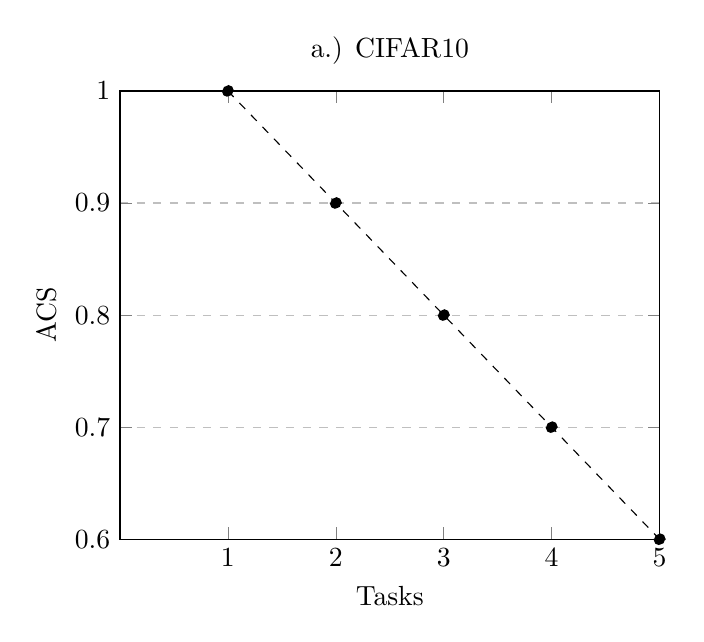
\begin{tikzpicture}
        \begin{axis}[
            title={a.) CIFAR10},
            xlabel={Tasks},
            ylabel={ACS},
            xmin=0, xmax=5,
            ymin=0.6, ymax=1,
            xtick={1,2,3,4,5},
            ytick={0.6,0.7,0.8,0.9,1},
            legend pos=north west,
            ymajorgrids=true,
            grid style=dashed,
        ]
        \addplot[
            color=black,
            mark=*,
            dashed,
        ]
        coordinates {
            (1, 1)
            (2, 0.9)
            (3, 0.8)
            (4, 0.7)
            (5, 0.6)
        };
        \end{axis}
    \end{tikzpicture}
    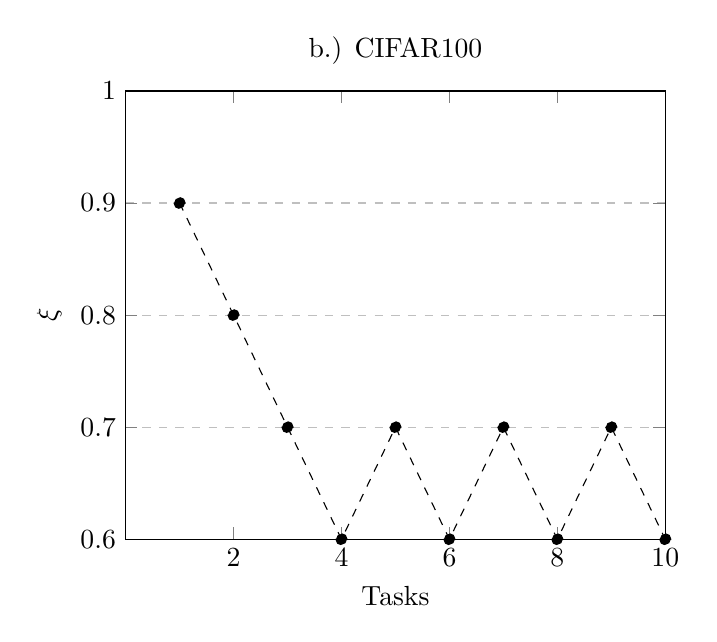
\begin{tikzpicture}
        \begin{axis}[
            title={b.) CIFAR100},
            xlabel={Tasks},
            ylabel={$\xi$},
            xmin=0, xmax=10,
            ymin=0.6, ymax=1,
            xtick={2,4,6,8,10},
            ytick={0.6,0.7,0.8,0.9,1},
            legend pos=north west,
            ymajorgrids=true,
            grid style=dashed,
        ]
        \addplot[
            color=black,
            mark=*,
            dashed,
        ]
        coordinates {
            (1, 0.9)
            (2, 0.8)
            (3, 0.7)
            (4, 0.6)
            (5, 0.7)
            (6, 0.6)
            (7, 0.7)
            (8, 0.6)
            (9, 0.7)
            (10, 0.6)
        };
        \end{axis}
    \end{tikzpicture}
    \caption{Illustrates the Average Confidence Score (ACS) for unlabeled data across tasks. The ACS calculated by taking average of maximum probability confidence scores from all the unlabeled data, at the end of training. The observed decaying trend indicates that using a fixed high threshold in SS-CIL may not be suitable for effective utilization of unlabeled data in feature learning. Due to the fixed threshold, the amount of unlabeled data utilized for training is significantly reduced as tasks progresses.}
    \label{fig:acs}
\end{figure}

\end{document}